\documentclass[../main.tex]{subfiles}

\begin{document}
\section{Linear models for regression}
The goal of regression is to predict the value of one or more continuous target variables $t$ given the value of
a D-dimensional vector $x$ of input variables. The simplest form of linear regression
models are also linear functions of the input variables. However, we can obtain a
much more useful class of functions by taking linear combinations of a fixed set of
nonlinear functions of the input variables, known as basis functions. Such models
are linear functions of the parameters, which gives them simple analytical properties,
and yet can be nonlinear with respect to the input variables. So the "linear" part in the title refers to the linearity respect to the parameters. So even though the model we are building is linear in the parameter space, it can estimate
nonlinear models in input/output space.

\subsection{Linear Basis Function Models}
\subsubsection{Linear regression}
The simplest linear model for regression is one that involves a linear combination of
the input variables. Given a set comprising M-1 observations ${x_m}$, where $m = 1, ..., M-1$ we have,
\begin{equation} \label{eqn_linear_basis}
    \begin{split}
         & y(x,w) = w_0+w_1x_1+...+w_{M-1}x_{M-1} = w_0+\sum_{n=1}^{M-1}(w_nx_n) = w^{T}x, \\
         &
        where \quad w^T=\begin{bmatrix}w_0 & w_1 & \dots & w_{M-1}\end{bmatrix},\quad
        x=\begin{bmatrix}1\\ x_1 \\ \vdots \\x_{M-1}\end{bmatrix}\footnotemark
    \end{split}
\end{equation}

This is often simply known as linear regression. The key
property of this model is that it is a linear function of the parameters $w_0, ..., w_{M-1}$. It is
also, however, a linear function of the input variables $x_i$, and this imposes significant limitations on the model.
\footnotetext{Note that we added a dummy sample $x_0=1$ to include $w_0$ in $w^{T}x$.}

\paragraph{Example} We want to estimate the weight of a person based on his age, height and gender
So our inputs variables would be
\begin{align*}
     & age,\quad     & x_a\in \mathbb{N} \\
     & height,\quad  & x_h\in \mathbb{N} \\
     & gender, \quad & x_g\in \mathbb{N} \\
     & bias, \quad   & 1
\end{align*}
\begin{align*}
    y(x,w)=
    \begin{bmatrix}w_0 & w_a & w_h & w_g\end{bmatrix}
    \begin{bmatrix}1\\ x_a \\ x_h \\x_g\end{bmatrix}
\end{align*}

\paragraph{Note} In linear regression we can distinguish two spaces. Hypothesis space(Parameters space) and Output space(Input space)

\begin{center}
    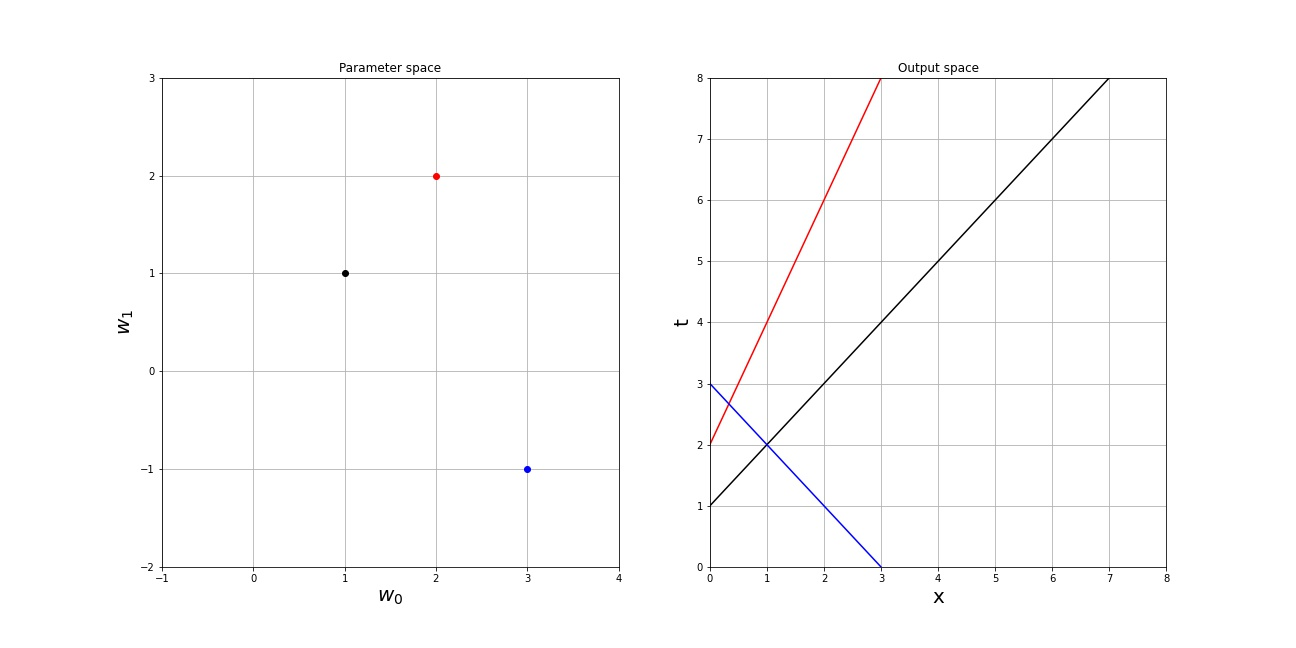
\includegraphics[scale=0.4]{images/param_input_space.jpg}
\end{center}

\subsubsection{Linear regression with non-linear basis functions}
We can extend the class of models by considering linear combinations of fixed nonlinear functions of the input variables, of the form
\begin{equation} \label{eqn_non-linear_basis}
    \begin{split}
         & y(x,w)=w_0+\sum_{j=1}^{M-1}(w_j\Phi_j(x))=w^T\Phi(x),                                   \\
         & where \quad \Phi(x)=\begin{bmatrix}1\\ \Phi_1(x) \\ \vdots \\\Phi_{M-1}(x)\end{bmatrix}
    \end{split}
\end{equation}
By using nonlinear basis functions\footnotemark, we allow the function $y(x,w)$ to be a nonlinear
function of the input vector $x$. Functions of the form (\ref{eqn_non-linear_basis}) are called linear
models because they are linear in w. It is this linearity in the parameters
that will greatly simplify the analysis of this class of models. From a geometric point of view the task of basis functions is to linearize input space "bending" the point into a straight line.

\footnotetext{Non-linear functions like: $e^x,sin(x),x^2$,...}

\subsubsection{Loss functions}
To evaluate which model, and so parameters, is the best, we need to quantify what it means to do well or poorly on a task. To do so we use loss functions.
\begin{align*}
     & L(t,y(x))                         & \text{Loss function}         \\
     & E[L]=\int\int L(t,y(x))p(x,t)dxdt & \text{Average loss function} \\
\end{align*}
Our goal is to find the model $y(x)$ that minimize the loss function $L(t,y(x))$.
If we take the Minkowsky loss
\begin{equation}
    \begin{split}
        E[L]=\int \int (t-y(x))^qp(t,x)dtdx
    \end{split}
\end{equation}
Based on $q$ the model that minimize $E[L]$ is
\begin{itemize}
    \item $q=2: \quad y(x) = E[t|x]$ Conditional mean. Note $E[t|x]=\int tp(t|x)dt$
    \item $q=1: \quad y(x) = median(t|x)$ Conditional median
    \item $q\xrightarrow{}0: \quad y(x) = mode(t|x)$ Conditional mode
\end{itemize}
\paragraph{Note} For $q=2$ we have the squared loss function. This is the most used one.

\subsection{Least square minimization}
The method of least squares is a standard approach in regression analysis to approximate a model by minimizing the sum of the squares of the residuals. Given N samples, we consider the following loss(error) function
\begin{equation}
    L(w)=\frac{1}{2}\sum_{n=1}^N(y(\underset{n^{th}input}{x_n},w)-\underset{n^{th}target}{t_n})^2
\end{equation}
This loss function is called SSE(Squared Sum of Errors) or half RSS(Residual Sum of Squares). It can be also written as
\begin{equation}
    RSS(w)=\|\epsilon\|_{2\quad l_2norm}^{2\quad square},\quad where \quad \epsilon=\begin{bmatrix}y(x_1,w)-t_1\\ \vdots \\ y(x_N,w)-t_N\end{bmatrix}
\end{equation}
\paragraph{Note} Given $x=\begin{bmatrix}x_1 & x_2 & \dots & x_{N}\end{bmatrix}$, the $l_2 norm$ of x corresponds to
\begin{align}
    l_2norm(x) = \|x\|_{2} = \sqrt{\sum_{n=1}^{N} x_n^2}
\end{align}

\newpage
\subsubsection{Ordinary Least Squares (Closed Form)}
Given N samples and M parameters, we construct $\Phi=\begin{bmatrix}\Phi(x_1) & \dots & \Phi(x_N)\end{bmatrix}^T$ and $t=\begin{bmatrix}t_1 & \dots & t_N\end{bmatrix}^T$.
\newline
We can rewrite the SSE in matrix notation
\begin{equation}
    %L(w) = \frac{1}{2}RSS(w)=\frac{1}{2}\underset{1x1}{\underset{(Nx1)^T}{(\underset{Nx1}{t}-\underset{NxM*Mx1}{\Phi w})^T}\underset{Nx1}{(\underset{Nx1}{t}-\underset{NxM*Mx1}{\Phi w})}}
    L(w) = \frac{1}{2}RSS(w)=\frac{1}{2}(t-\Phi w)^T(t-\Phi w) \quad [1 \times 1]\footnotemark
\end{equation}

\paragraph{Note} $\Phi[N \times M]$, $w[M \times 1]$, $t[N \times 1]$
\footnotetext{The [ ] next to the equations indicates result dimensions}
\newline
To minimize L(w) we have to calculate the first and the second derivative
\begin{equation}
    \frac{\partial L(w)}{\partial w}=\frac{\partial(\frac{1}{2}(t-\Phi w)^T(t-\Phi w))}{\partial w} = -\Phi^T(t-\Phi w) \quad[M \times 1]
\end{equation}

\paragraph{Note} $\frac{\partial L(w)}{\partial w}$ are the directions of every $w_i$ to minimize $L(w)$

\begin{equation}
    \frac{\partial L(w)}{\partial w \partial w^T}=\Phi^T\Phi \quad [M \times M]
\end{equation}

\paragraph{Note} $\frac{\partial L(w)}{\partial w \partial w^T}$ is a semi-definite positive matrix\footnotemark, so all eigen values$\geq0$. It also means that for $\frac{\partial L(w)}{\partial w}=0$ we find the minimum of $L(w)$

\footnotetext{$x^T\Phi^T \Phi x\geq0,\quad \forall x\in \mathbb{R} \setminus \emptyset$}

Now we have to find $w$ imposing the first derivative to zero

\begin{align*}
    \frac{\partial L(w)}{\partial w} & =0                                                       \\
    -\Phi^T(t-\Phi w)                & =0                                                       \\
    -\Phi^Tt+\Phi^T\Phi w            & =0                                                       \\
    \Phi^T\Phi w                     & =\Phi^Tt                                                 \\
    \hat{w}                          & =(\Phi^T\Phi)^{-1}\Phi^Tt \quad [M \times 1] \numberthis
\end{align*}

Second derivative can give us some infos about features(basis functions) importance. If we have some eigen values close to zero we could have the following situations
\begin{itemize}
    \item $N<M$, less samples than dimensions(parameters)
    \item The feature with null eigen value is linearly dependents from other features
\end{itemize}
From a computational point of view the matrix invertion is a very complex operation. In fact, the temporal complexity of OLS is
\begin{align*}
    O(NM^2+M^3)
\end{align*}

\newpage
\paragraph{Geometric interpretation}
We can give a geometric interpretation of the problem. Given $\hat{t}=\begin{bmatrix}y(x_1,w) & \dots & y(x_N,w)\end{bmatrix}^T$ from the previous calculation we can say that $\hat{t}$ is a linear combination of the column of $\Phi$. So $\hat{t}$ lies in a M-subspace S and since $\hat{t}$ minimize $L(w)$ with respect to $t$, it represents the projection of $t$ in S
\begin{align*}
    %\hat{t}=\underbrace{\Phi(\Phi^T\Phi)^{-1}\Phi^T}_{\text{Hat matrix H}}t=Ht, \quad \text{H projects t on S}
    \hat{t}=\underbrace{\Phi(\Phi^T\Phi)^{-1}\Phi^T}_{\text{Hat matrix H}}t=Ht, \quad \text{H projects t on S}
\end{align*}

\subsubsection{Maximum Likelihood ML (Closed Form)}
We assume that the target variable t is given by a deterministic function
$f(x)$ with additive Gaussian noise $\epsilon$ so that
\begin{align*}
    t=f(x)+\epsilon
\end{align*}
To estimate $t$ we can make the following assumptions
\begin{itemize}
    \item Approximate $f(x)$ with $y(x,w)$
    \item Assume $\epsilon\sim\mathcal{N}(0, \sigma^2)$
\end{itemize}
Given N i.i.d.\footnotemark samples, with input $X=\{x_1,...,x_N\}$ and outputs $t=\begin{bmatrix} t_1 & \dots & t_N\end{bmatrix}^T$ we can say that
\begin{align}
    t_i\sim \mathcal{N}(t_i|w^T\Phi(x_i),\sigma^2)
\end{align}
\footnotetext{Independent and Identically Distributed random variables}
For the properties of the Gaussian distribution we can write the following
\begin{align*}
    p(t|X,w,\sigma^2)      & =\prod_{n=1}^N \mathcal{N}(t_n|w^T\Phi(x_n),\sigma^2)                                                                                     \\
    p(t|X,w,\sigma^2)      & =\prod_{n=1}^N\frac{1}{\sqrt{2\pi}\sigma}e^{-\frac{1}{2}\frac{(t_n-w^T\Phi(x_n))^2}{\sigma^2}}                                            \\
    \Downarrow \quad \quad & \text{Transition to ln to simplify calculus.}                                                                                             \\
                           & \text{Min \& Max remain the same}                                                                                                         \\
    ln(p(t|X,w,\sigma^2))  & =ln\prod_{n=1}^N\frac{1}{\sqrt{2\pi}\sigma}e^{-\frac{1}{2}\frac{(t_n-w^T\Phi(x_n))^2}{\sigma^2}}                                          \\
                           & =\sum_{n=1}^Nln\bigg( \frac{1}{\sqrt{2\pi}\sigma}e^{-\frac{1}{2}\frac{(t_n-w^T\Phi(x_n))^2}{\sigma^2}} \bigg)                             \\
                           & =\sum_{n=1}^Nln\bigg(\frac{1}{\sqrt{2\pi}\sigma}\bigg) + ln\bigg(e^{-\frac{1}{2}\frac{(t_n-w^T\Phi(x_n))^2}{\sigma^2}}\bigg)              \\
                           & =\sum_{n=1}^Nln\bigg(\frac{1}{\sqrt{2\pi}\sigma}\bigg) + \sum_{n=1}^N ln\bigg(e^{-\frac{1}{2}\frac{(t_n-w^T\Phi(x_n))^2}{\sigma^2}}\bigg) \\
                           & =\sum_{n=1}^Nln\bigg(\frac{1}{\sqrt{2\pi}\sigma}\bigg) + \sum_{n=1}^N -\frac{1}{2}\frac{(t_n-w^T\Phi(x_n))^2}{\sigma^2}                   \\
                           & =\sum_{n=1}^Nln\bigg(\frac{1}{\sqrt{2\pi}\sigma}\bigg) -\frac{1}{2\sigma^2} \sum_{n=1}^N(t_n-w^T\Phi(x_n))^2                              \\
                           & =\sum_{n=1}^Nln\bigg((2\pi\sigma^2)^{-\frac{1}{2}}\bigg) -\frac{1}{2\sigma^2} \sum_{n=1}^N(t_n-w^T\Phi(x_n))^2                            \\
                           & =-\frac{N}{2}ln(2\pi\sigma^2) -\frac{1}{2\sigma^2} \underbrace{\sum_{n=1}^N(t_n-w^T\Phi(x_n))^2}_{RSS} \numberthis
\end{align*}
To find the maximum likelihood, we equal the gradient of $ln(p(t|X,w,\sigma^2))=0$
\begin{align*}
    \overset{w}{\nabla}ln(p(t|X,w,\sigma^2)) & =\overset{w}{\nabla}\bigg( -\frac{1}{2\sigma^2} \sum_{n=1}^N(t_n-w^T\Phi(x_n))^2 \bigg)                            \\
                                             & =-\frac{1}{2\sigma^2} \sum_{n=1}^N2(t_n-w^T\Phi(x_n))(-\Phi^T(x_n))                                                \\
                                             & =-\frac{1}{\sigma^2} \sum_{n=1}^N t_n\Phi^T(x_n) - w^T \sum_{n=1}^N \Phi(x_n)\Phi^T(x_n)                           \\
    0                                        & = \sum_{n=1}^N t_n\Phi^T(x_n) - w^T \sum_{n=1}^N \Phi(x_n)\Phi^T(x_n)                                              \\
    w^T                                      & = \sum_{n=1}^N t_n\Phi^T(x_n) \bigg( \sum_{n=1}^N \Phi(x_n)\Phi^T(x_n) \bigg)^{-1}                                 \\
    w                                        & = \bigg( \sum_{n=1}^N t_n\Phi^T(x_n) \bigg( \sum_{n=1}^N \Phi(x_n)\Phi^T(x_n) \bigg)^{-1} \bigg)^T                 \\
                                             & = \bigg( \bigg( \sum_{n=1}^N \Phi(x_n)\Phi^T(x_n) \bigg)^{-1} \bigg)^T \bigg( \sum_{n=1}^N t_n\Phi^T(x_n) \bigg)^T \\
                                             & = \bigg( \sum_{n=1}^N \Phi(x_n)\Phi^T(x_n) \bigg)^{-1} \sum_{n=1}^N \Phi(x_n)t_n
    \quad \quad having \quad \Phi=\begin{bmatrix} \begin{bmatrix} \Phi^T(x_1) \end{bmatrix} \\ \vdots \\ \begin{bmatrix} \Phi^T(x_N) \end{bmatrix} \end{bmatrix}                                \\
                                             & = (\Phi^T \Phi)^{-1} \Phi^T t \quad [M \times 1] \numberthis \label{ML_result}
\end{align*}

\newpage
As we can see both OLS and ML give the same result (\ref{ML_result}).

\paragraph{W variance estimation} As we said before for ML calculation we made some assumptions. The most important for calculating the variance are:
\begin{itemize}
    \item the observations $t_i$ are uncorrelated and have constant variance $\sigma^2$
    \item $x_i$ are fixed(non-random)
\end{itemize}
Given that the variance-covariance matrix of least-squares estimates is
\begin{equation}
    Var(\hat{w}_{ML})=(\Phi^T\Phi)^{-1}\sigma^2
\end{equation}
As we have seen before $\Phi^T\Phi$ matrix can give us some insights on features importance. If a features is relevant its eigen value is high. An effect of this is the reduction of parameters variance. In fact the $\Phi^T\Phi$ matrix is inverted(same as divided) and multiplied to error variance $\sigma$, so high eigen values reduce variance.
We can achieve variance reduction by gathering more samples for our estimation.

\paragraph{Multiple outputs} To solve a regression problem with multiple outputs we could use different sets of basis function for each output, having independents problems. Usually, a single set of basis function is used
\begin{equation}
    \hat{W}_{ML}=\underbrace{(\Phi^T\Phi)^{-1}\Phi^T}_{\Phi^{\dagger} \text{Pseudo-inverse}} T\quad [M \times K],\quad where \quad T \quad [N \times K]
\end{equation}

\subsubsection{Gradient optimization (Open form)}
Closed-form solutions are not practical with large datasets because they are computationally too complex. To overcome this problem, we can use iterative approaches which make sequential (online) updates of the parameters instead of calculating them directly. An example is stochastic\footnotemark{} gradient descent.
\footnotetext{Stochastic means that we won't use all data at once to update the parameters, but we can update them from smaller subsets of the dataset. This is done to reduce the complexity.}
If the loss function can be represented as a sum over samples ($L(x)=\sum_nL(x_n)$) this iterative approach is applicable. This is the case for least squares.
\begin{align}
    w^{\overset{\text{iteration}}{(k+1)}}=w^{(k)}-\underset{\text{learning rate}}{\alpha^{(k)}} \nabla L(x_n)
\end{align}
The learning rate $\alpha$ is an important hyperparameter\footnotemark \footnotetext{In machine learning, a hyperparameter is a parameter whose value is used to control the learning process. By contrast, the values of other parameters are derived via training.}of the model. It defines the length of each iteration step. A big step makes the iterative process converge faster, but is less precise because it can "jump" the minimum that we are looking for. Similarly if we take small steps we are more precise but we could get stuck in local minima and the convergence is slow. To be sure of algorithm convergence the learning rate must have the following properties
\begin{equation}
    \sum_{k=0}^{\infty}\frac{1}{\alpha^{(k)}}=\infty \quad \wedge \quad \sum_{k=0}^{\infty}\frac{1}{{\alpha^{(k)}}^2}=M, \quad M\in\mathbb{R}
\end{equation}

\subsubsection{Underfitting - Overfitting} \label{fitting}
Model complexity play a very important role for the success of an algorithm. A simple definition of 'model complexity' can be define as the number of parameters and features of a model. The complexity influence model capability to generalize.
An optimal model is one that generalize well the problem and generalization is the model’s ability to give sensible outputs to sets of input that it has never seen before. We can have either two cases for bad generalization.
\begin{itemize}
    \item \textbf{Underfitting} The model is too simple and it generalize too much. In practice we don't have enough parameter to estimate the true model.
    \item \textbf{Overfitting} The model is too complex and it relies too much on the given dataset. The model will behave very well on our dataset, but will perform poorly on other ones. In practice the model tries to interpolate the dataset learning the true model and the noise of our starting dataset because it has too many parameters.
\end{itemize}
A naive way to measure the performance of our model is to look at the loss function value. A lower value corresponds to a better performance. This is true, but loss function value lacks of valuable information regarding model complexity. In fact, as we had said before, an overfitting model tries to interpolate the dataset, this will produce a loss function value that tends to zero but the model true performance is far from optimal.
\begin{center}
    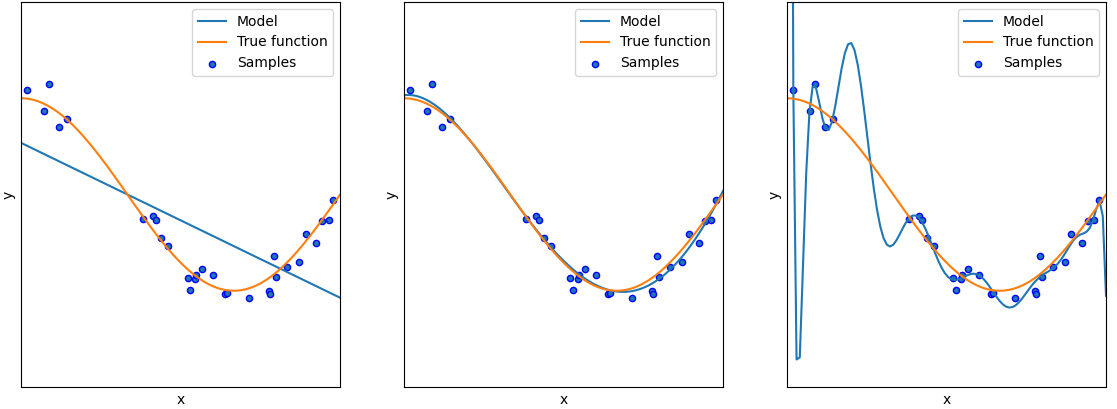
\includegraphics[scale=0.5]{images/Under-Overfitting.png}
\end{center}
To overcome this problem we can split the dataset in two subset,
\begin{itemize}
    \item \textbf{Training set} This set is used to learn the model's parameters.
    \item \textbf{Test set} This set is used to test model performance on unseen data. This is very helpful for complexity selection.
\end{itemize}
A good error function for testing the complexity is
\begin{equation}
    E_{RMS}=\sqrt{\frac{2RSS(\hat{w})}{N}}
\end{equation}
Differently from the loss function used at training time $E_{RMS}$ is not monotonically decreasing with model complexity. It has a U shape and the minimum corresponds to the optimal model complexity.

\begin{center}
    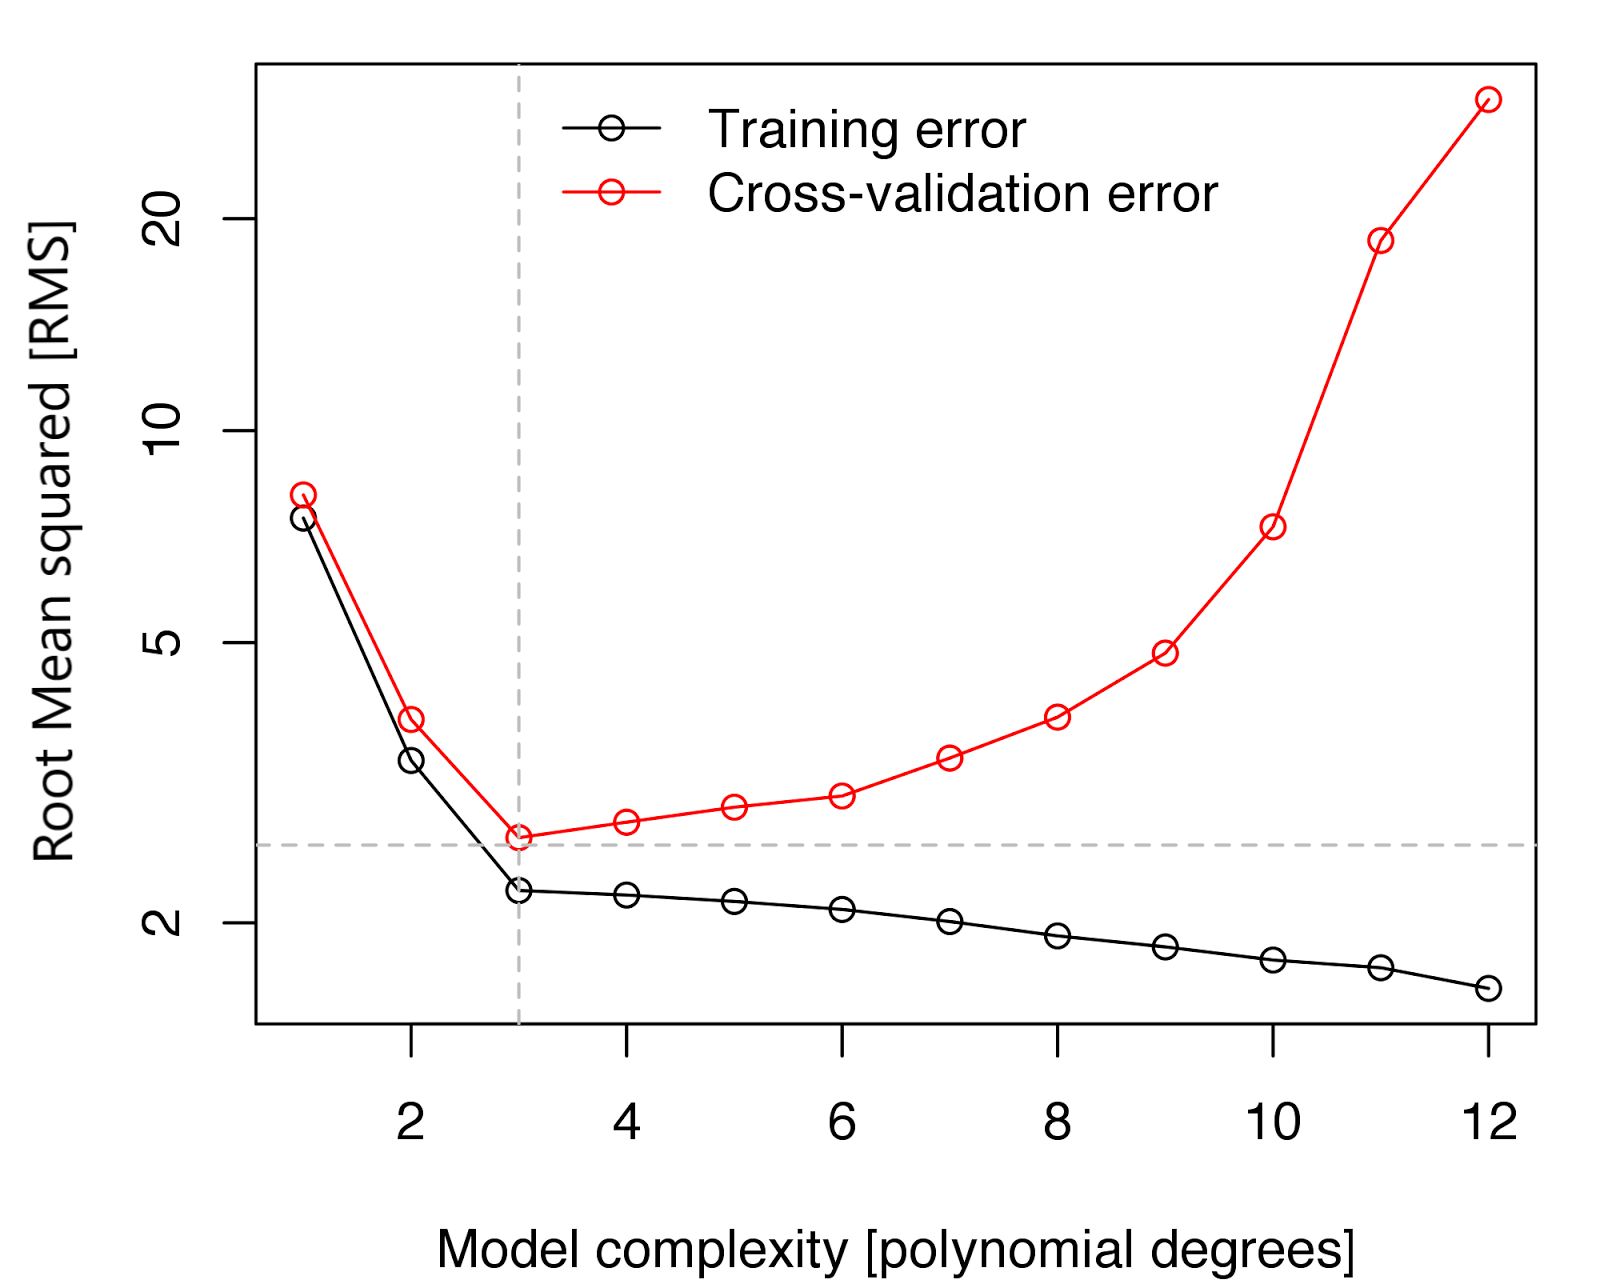
\includegraphics[scale=0.25]{images/error_complexity.png}
\end{center}

Another indicator for poor generalization is parameters absolute value. If we have very large parameters it means that the model oscillate very rapidly. This is an evidence of overfitting.

\subsection{Regularization}
One of the major aspects of training your machine learning model is avoiding overfitting. The model will have a low accuracy if it is overfitting. This happens because your model is trying too hard to capture the noise in your training dataset. One way to avoid overfitting is using cross validation. Another way to reduce overfitting is constrain/regularize or shrink the parameters estimates towards zero. To do so, we can change the loss function
\begin{equation}
    L(w)=\underbrace{L_D(w)}_{\text{error on data}}+ \underbrace{\lambda L_W(w)}_{\text{error on complexity}}
\end{equation}
For tractability we take
\begin{align*}
     & L_D(w)=\frac{1}{2}RSS & L_W(w)=\frac{1}{2}\sum_{j=1}^M |w_j|^q, \quad q\in\mathbb{N}^+
\end{align*}
As we can see $L_W$ depends on parameter absolute value. This loss function component discourages high parameters values. So a parameters have to justify its high value by giving a very good contribution to $L_D$, otherwise the model is penalized.
The penalization of $L_W$ can be controlled with $\lambda$(regularization coefficient) and $q$.
Furthermore we can interpret $L_W$ as a constraint. If we consider the parameters space, $L_w$ is bounding the parameters at a certain distance from the origin. The distance is imposed by $\lambda$ and $q$. In particular, $q$ modifies the shape of the boundary(constraint) in the parameters space.
The most used value for $q$ are $1$ and $2$.
\begin{center}
    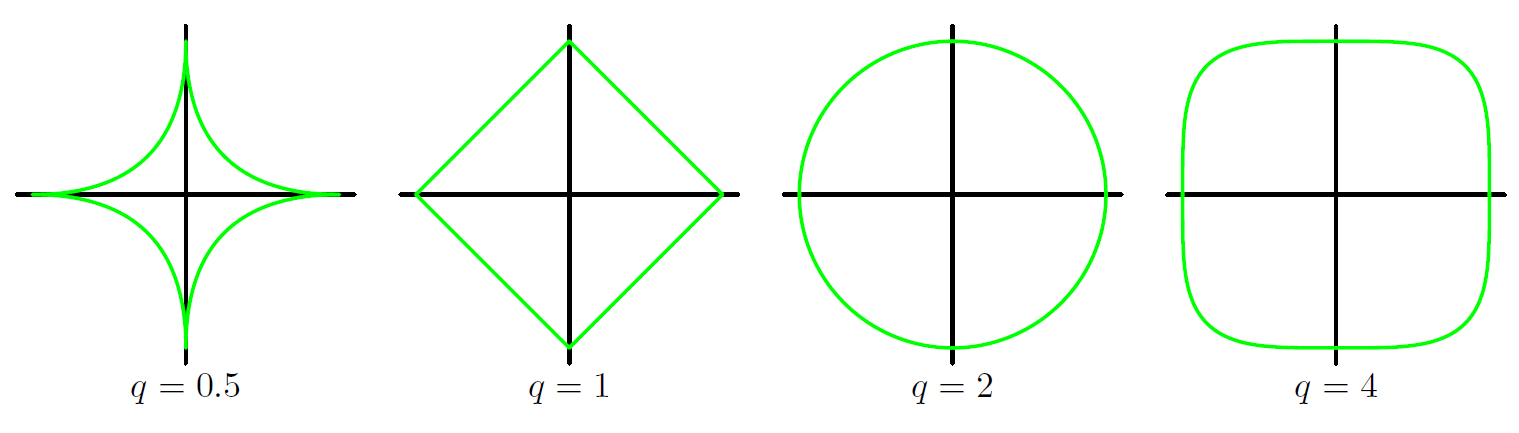
\includegraphics[scale=0.4]{images/Q_boundaries_regularization.PNG}
\end{center}
Regularization allows complex models to be trained on data sets of limited size
without severe over-fitting, essentially by limiting the effective model complexity.
However, the problem of determining the optimal model complexity is then shifted
from one of finding the appropriate number of basis functions to one of determining
a suitable value of the regularization coefficient $\lambda$.

\subsubsection{Ridge regression}
For $q=2$ we have the so called Ridge regression.
\begin{align*}
    L_W(w) & =\frac{1}{2}w^T w = \frac{1}{2}\| w \|_2^2                              \\
    L(w)   & = \frac{1}{2}\sum_{j=1}^N(t_i-w^T\Phi(x_i))^2 + \frac{\lambda}{2}w^T w  \\
           & =\frac{1}{2}(t-\Phi w)^T(t-\Phi w) + \frac{\lambda}{2}w^T w \numberthis
\end{align*}
The main advantage of ridge regression is that the loss function is still quadratic in w, so we can still derive a closed form solution.
\begin{equation}
    \hat{w}_{ridge}=(\lambda I+\Phi^T \Phi)^{-1}\Phi^T t
\end{equation}
\paragraph{Note} The eigen values of $(\lambda I+\Phi^T \Phi)$ are still greater or equal to zero because $\Phi^T \Phi$ is semi-definite positive and $\lambda I$ simply imposes a positive lower bound to the eigen values. $(\lambda I+\Phi^T \Phi)$ is still semi-definite positive and so invertible.

\subsubsection{Lasso}
For $q=1$ we have the so called Lasso.
\begin{align*}
    L_W(w) & = \frac{1}{2}\sum_{j=1}^M |w_j| = \frac{1}{2}\| w \|_1                                 \\
    L(w)   & = \frac{1}{2}\sum_{j=1}^N(t_i-w^T\Phi(x_i))^2 + \frac{\lambda}{2}\sum_{j=1}^M |w_j|    \\
           & = \frac{1}{2}\sum_{j=1}^N(t_i-w^T\Phi(x_i))^2 + \frac{\lambda}{2}\| w \|_1 \numberthis
\end{align*}
Differently from ridge regression, lasso is not linear. No closed form solution exists because we have the absolute value operator in $L_W$. In contrast, a very good advantage is the capability to make some weights equal to zero for values of $\lambda$ large enough. This means that lasso leads to sparser models\footnotemark.
\footnotetext{A model is sparse if some parameters tend to zero, eliminating some features from the model}
\begin{center}
    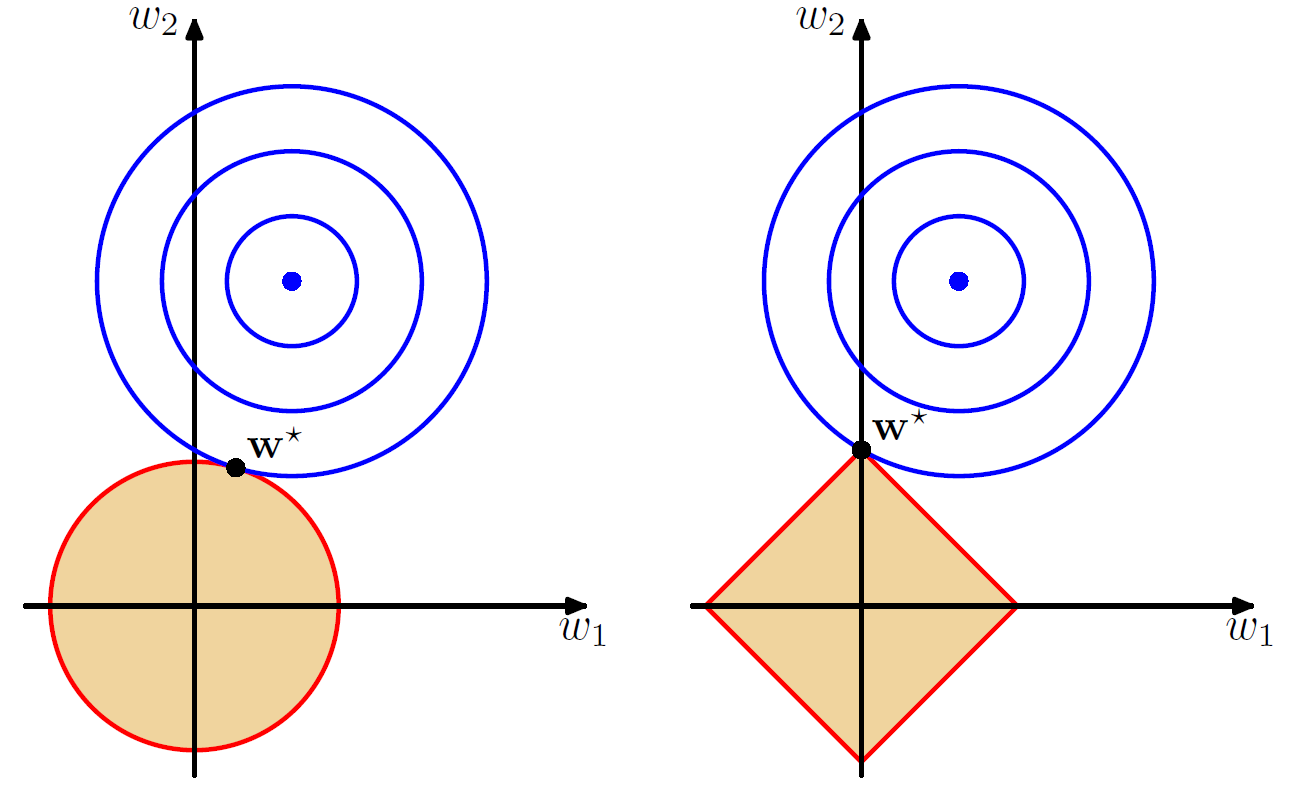
\includegraphics[scale=0.4]{images/Parameter_space_regularization.PNG}
\end{center}
The red lines in the figure represents $\sum_{j=1}^M |w_j|^q$ respectively for $q=2$ and $q=1$.
The blue lines are the unregularized error functions.
\newpage

\subsection{Bayesian Linear regression}
In our discussion of maximum likelihood for setting the parameters of a linear regression
model, we have seen that the effective model complexity, governed by the
number of basis functions, needs to be controlled according to the size of the data
set. Adding a regularization term to the log likelihood function means the effective
model complexity can then be controlled by the value of the regularization coefficient,
although the choice of the number and form of the basis functions is of course
still important in determining the overall behaviour of the model.
This leaves the issue of deciding the appropriate model complexity for the particular
problem, which cannot be decided simply by maximizing the likelihood function,
because this always leads to excessively complex models and over-fitting. We therefore turn to a Bayesian treatment of linear regression, which will
avoid the over-fitting problem of maximum likelihood, and which will also lead to
automatic methods of determining model complexity using the training data alone.

\paragraph{Note} Bayes theorem is obviously the hearth of this type of regression. As a reminder, Bayes theorem states
\begin{equation}
    \underbrace{P(A|B)}_{Posterior} = \frac{\overbrace{P(B|A)}^{Likelihood} \overbrace{P(A)}^{Prior}}{\underbrace{P(B)}_{Marginalization}}
\end{equation}

\paragraph{Example} We can estimate the probability of getting head or tail with a coin flip. We don't know if the coin is tricked or not.
We know that a coin flip follow a Bernoulli distribution
\begin{align*}
    P(r)=
    \begin{cases}
        p,     & \text{if } r = \text{Head} \\
        q=1-p, & \text{if } r = \text{Tail}
    \end{cases}
\end{align*}
\begin{itemize}
    \item \textbf{Prior} $P(r)$ we assume a regular coin so $P(r) = p = \frac{1}{2}$ ($P(Head)=\frac{1}{2}$ and $P(Tail)=\frac{1}{2}$)
    \item \textbf{Posterior} $P(r|D)$ Probability of the coin having $p=\frac{1}{2}$ given the Data.
    \item \textbf{Likelihood} $P(D|r)$ Probability of observing the Data given that the coin have $P=\frac{1}{2}$
    \item \textbf{Marginalization} $P(D)$ Probability of observing the Data
\end{itemize}
\begin{equation*}
    P(r|D) = \frac{P(D|r)P(r)}{P(D)}
\end{equation*}
So the Bayesian approach formulate our knowledge as follow,
\begin{enumerate}
    \item We formulate our knowledge about the world in a probabilistic way
          \begin{enumerate}
              \item We define the model that expresses our knowledge qualitatively
              \item We capture our assumptions about unknown parameters by specifying the
                    prior distribution over those parameters before seeing the data
          \end{enumerate}
    \item We observe the data
    \item We compute the posterior probability distribution for the parameters, given observed data
    \item We use the posterior distribution to make predictions or take decisions
\end{enumerate}

As the example we have made before we have
\begin{equation*}
    P(w|D) = \frac{P(D|w)P(w)}{P(D)}
\end{equation*}
\begin{itemize}
    \item \textbf{Prior} $P(w)$ probability distribution of the parameters
    \item \textbf{Posterior} $P(w|D)$ Probability of w given training data D
    \item \textbf{Likelihood} $P(D|w)$ Probability of observing the Data given parameters w
    \item \textbf{Marginalization} $P(D)$ Probability of observing the Data $P(D)=\int P(D|w)P(w)dw$
\end{itemize}
Our objective is to find the most probable value of $w$ given the data maximum a
posteriori (MAP), which is the mode of the posterior $P(w|D)$.

\paragraph{Note} An advantage of the Bayesian approach is the introduction of the prior distribution. This greatly reduce our hypothesis space(parameter space) reducing overfitting.
Assuming a Gaussian likelihood model we can take a Gaussian prior.
The Gaussian family is conjugate to itself (or self-conjugate) with respect to a Gaussian likelihood function: if the likelihood function is Gaussian, choosing a Gaussian prior over the mean will ensure that the posterior distribution is also Gaussian.
\begin{equation}
    P(w) \sim \mathcal{N} (w|w_0, S_0)
\end{equation}
\begin{itemize}
    \item $w_0$ $[M \times 1]$ Mean of the distribution. We guess that $w$ is equal to $w_0$ in the parameter space.
    \item $S_0$ $[M \times M]$ Covariance matrix of the distribution. The matrix is diagonal because we assume i.i.d. parameters.
\end{itemize}
So P(w) is a multivariate\footnotemark Gaussian.
\footnotetext{In probability theory and statistics, the multivariate normal distribution or multivariate Gaussian distribution is a generalization of the one-dimensional (univariate) normal distribution to higher dimensions.}
As we have said before, the posterior will be Gaussian
\begin{align*}
    P(w|t, \Phi, \sigma^2) & \propto \mathcal{N} (w|w_0, S_0) \mathcal{N} (t|\Phi w, \sigma^2I_N) = \mathcal{N} (w_N,S_N) \\
    w_N                    & = S_N \bigg( S_0^{-1}w_0 + \frac{\Phi^T t}{\sigma^2} \bigg)                                  \\
    S_N^{-1}               & = S_0^{-1} + \frac{\Phi^T \Phi}{\sigma^2}
\end{align*}

\newpage
For two particular prior distribution cases, Bayesian regression estimate reduces to already known regressions,
\begin{itemize}
    \item $S_0 = \infty I$
          In this case we have no prior knowledge of the parameters distribution. If we substitute $S_0$ in $w_N$ definition we find,
          \begin{align*}
              S_N^{-1} & = S_0^{-1} + \frac{\Phi^T \Phi}{\sigma^2}
              = \frac{\Phi^T \Phi}{\sigma^2}                                                 \\
              S_N      & = \sigma^2 (\Phi^T \Phi)^{-1}                                       \\
              w_N      & = S_N \bigg( S_0^{-1}w_0 + \frac{\Phi^T t}{\sigma^2} \bigg)         \\
                       & = \sigma^2 (\Phi^T \Phi)^{-1} \frac{\Phi^T t}{\sigma^2}             \\
                       & = (\Phi^T \Phi)^{-1} \Phi^T t \numberthis \label{eqn_bayes_inf_var}
          \end{align*}
          As we can see (\ref{eqn_bayes_inf_var}) is equal to the ML estimator. So Bayesian regression reduces to the maximum likelihood case.
    \item $w_0 = 0$, $S_0 = \tau^2 I, \quad \tau \in \mathbb{R}$
          \begin{align*}
              S_N^{-1} & = S_0^{-1} + \frac{\Phi^T \Phi}{\sigma^2}                                                              \\
                       & = \frac{1}{\tau^2}I + \frac{\Phi^T \Phi}{\sigma^2}                                                     \\
              w_N      & = S_N \bigg( S_0^{-1}w_0 + \frac{\Phi^T t}{\sigma^2} \bigg)                                            \\
                       & = S_N \frac{\Phi^T t}{\sigma^2}                                                                        \\
                       & = \bigg( \frac{1}{\tau^2}I + \frac{\Phi^T \Phi}{\sigma^2} \bigg)^{-1} \frac{\Phi^T t}{\sigma^2}        \\
                       & = \bigg( \frac{\sigma^2}{\tau^2}I + \Phi^T \Phi \bigg)^{-1} \Phi^T t \numberthis \label{eqn_bayes_0_w}
          \end{align*}
          We can notice that (\ref{eqn_bayes_0_w}) is equal to Ridge regression with $\lambda=\frac{\sigma^2}{\tau^2}$. Small values of $S_0$ corresponds to high values of $\lambda$ and viceversa.
\end{itemize}

\newpage
\paragraph{Example - Bayesian sequential learning}
We generate some data from
\begin{equation*}
    t(x) = -0.3 + 0.5x + \epsilon, \quad where \quad \epsilon \sim \mathcal{N}(0,0.04)
\end{equation*}
As a model we take
\begin{equation*}
    y(x,w) = w_0+w_1x, \quad \sigma^2=0.04, \quad \tau^2=0.5
\end{equation*}
To find the posterior distribution we use an iterative approach as follow.
We start from a multivariate Gaussian prior $P(w) \sim \mathcal{N}(0,\tau^2 I)$ (prior). Then we take one data point and we find the parameters that make the model pass through that point, also considering data noise $\sigma^2$ (likelihood). The next step is to multiply the prior with the likelihood to find a posterior distribution in parameters space. The new posterior can be used as a prior for the next iteration. We take a new point, we find the parameters that make the model pass through that point and again we multiply together prior and likelihood. Note that at each iteration, the likelihood distribution considers only one point at the time.
\begin{center}
    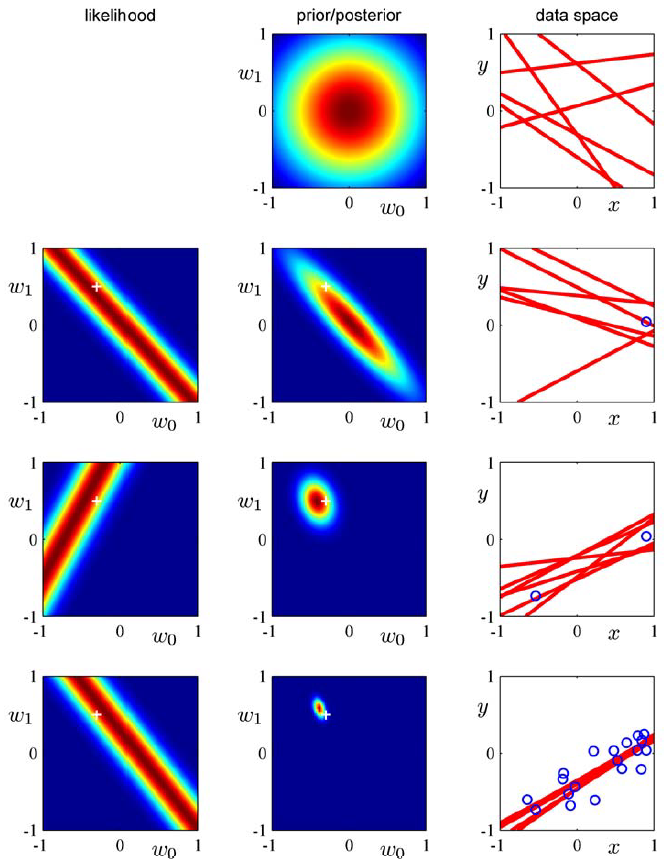
\includegraphics[scale=0.6]{images/Bayes_sequential.PNG}
\end{center}

\newpage
\subsubsection{Predictive distribution}
In practice, we are not usually interested in the value of w itself but rather in
making predictions of t for new values of x. This requires that we evaluate the posterior predictive distribution defined by,
\begin{align*}
    p(t|x,D,\sigma^2) & = \int \mathcal{N}(t|w^T\Phi(x),\sigma^2) \mathcal{N}(w|w_N, S_N)dw = \mathcal{N}(t|w_N^T\Phi(x), \sigma_N^2(x)), \numberthis \\
    \sigma_N^2(x)     & = \underbrace{\sigma^2}_{\substack{\text{noise in the}                                                                        \\ \text{target values}}} + \underbrace{\Phi(x)^T S_N \Phi(x)}_{\substack{\text{Uncertainty associated} \\ \text{with parameters values}}} \numberthis
\end{align*}
$\sigma^2$ is also called irreducible noise, in fact for $N \rightarrow \infty$, the second term of $\sigma_N^2(x)$ goes to zero, but $\sigma^2$ remain constant.
In the figure below we can observe,
\begin{itemize}
    \item \textbf{Green line} True model
    \item \textbf{Blue dots} Samples
    \item \textbf{Red line} Mean of the Gaussian predictive distribution
    \item \textbf{Red area} Predictive distribution spanning one standard deviation either side of the mean.
\end{itemize}

\begin{center}
    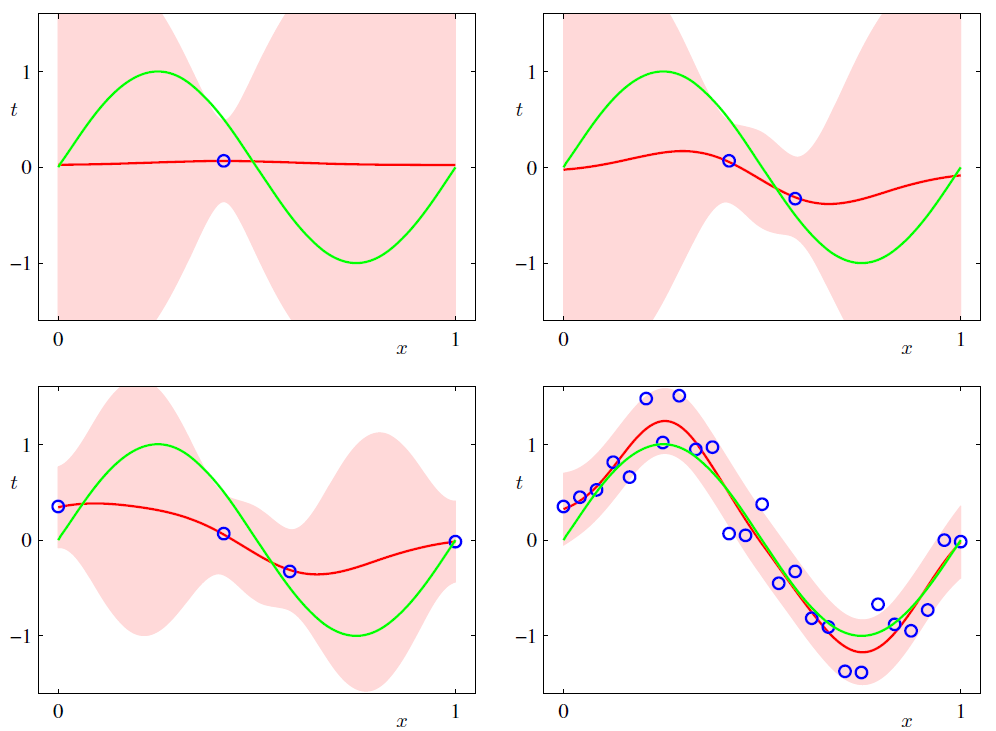
\includegraphics[scale=0.6]{images/Posterior_predictive_distribution.PNG}
\end{center}

\end{document}